\documentclass{article}
\usepackage{tikz}

\begin{document}

% Define colors used in the figure
\definecolor{gray}{RGB}{153,153,153}
\definecolor{teal}{RGB}{0,128,128}

% Set up the TikZ environment
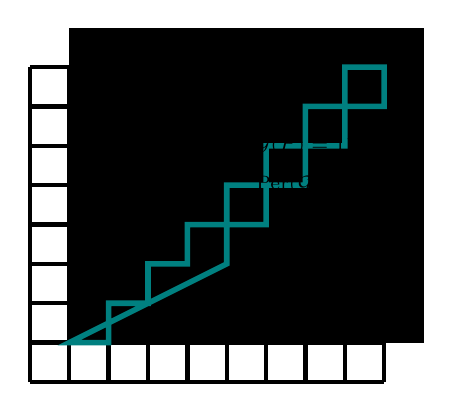
\begin{tikzpicture}[scale=0.5]
    % Draw the grid
    \draw[ultra thick] (-1,-1) grid (8,7);
    
    % Highlight the gray cluster
    \foreach \i in {0,1,...,8}{
        \foreach \j in {0,1,...,7}{
            \pgfmathparse{\i>\j || \i<\j ? "gray" : "white"}
            \edef\color{\pgfmathresult}
            \fill[\color] (\i,\j) rectangle ++(1,1);
        }
    }
    
    % Highlight the teal perimeter
    \draw[line width=2pt,teal] 
        (0,0) -- (1,0) -- (1,1) -- (2,1) -- (2,2) -- (3,2) -- (3,3) -- (4,3) -- (4,4) -- (5,4) -- (5,5) -- (6,5) -- (6,6) -- (7,6) -- (7,7) -- (8,7) -- (8,6) -- (7,6) -- (7,5) -- (6,5) -- (6,4) -- (5,4) -- (5,3) -- (4,3) -- (4,2) -- cycle;
    
    % Add labels for the cluster and perimeter information
    \node at (4.5,6.5) {$\mathcal{G}(P)$};
    \node at (4.5,5.5) [below right] {\scriptsize $\abs{\mathcal{G}(P)} = 11$};
    \node at (4.5,4.5) [below right] {\scriptsize $\mathrm{Per}(\mathcal{G}(P)) = 19$};
    
\end{tikzpicture}

\end{document}